\section{Přenosové vlastnosti optických vláken, vlákna mnohovidová a jednovidová, polymerová optická vlákna (POF).}

\subsection{Vlastnosti}
Výhody:
\begin{itemize}
    \item vysoká přenosová kapacita
    \item nevyzařování z kabelů (žádné přeslechy)
    \item menší rozměry a hmotnost
    \item v mnoha případech není potřeba opakovačů
    \item spolehlivý přenos
\end{itemize}
Nevýhody:
\begin{itemize}
    \item problémy při spojování
    \item vydělovaní signálů
    \item náchylnost na ohyb
\end{itemize}

\subsection{Mnohavidová vlákna}
\subsubsection{Mnohovidové s konstantním indexem lomu jádra}
Vyznačují jednoduchou výrobou a manipulací, v poměrně jednoduchém konstruování, nevýhodou ve větším útlumu, disperzi a malé přenosové kapacitě. Vyznačují se většími průměry jádra a pláště.

Vlákna tohoto typu jsou nejvíce využívána pro spoje na krátké vzdálenosti, především pro automatizační účely, krátké přenosy dat, lokální sítě apod. 

\begin{figure}[!ht]
\begin{center}
    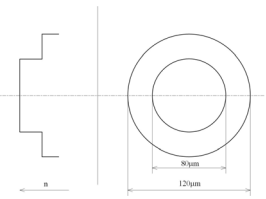
\includegraphics[scale=1]{obrazky/mnohavid1.png}
  \end{center}
\end{figure}

\begin{figure}[!ht]
\begin{center}
    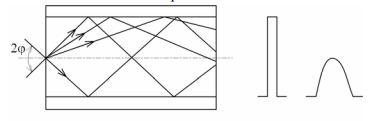
\includegraphics[scale=1]{obrazky/sirmnoh1.png}
  \end{center}
\end{figure}

Některé charakteristiky tohoto typu vlákna: Průměr jádra = 50 – 200µm, Průměr pláště = 120 - 300µm, disperze 50 ns/km, útlum 5 – 20 dB/km, šířka pásma 60 Mbit. 

\subsubsection{Mnohovidové vlákno s proměnným indexem lomu jádra (gradientní)}
Vyznačují menší disperzí, menším útlumem, částečně složitější výrobou a tím složitějším konstruováním a spojováním vláken. Vlákno je normalizováno dle doporučení ITU-T, průměr jádra = 50µm, průměr pláště = 125µm.

Tento typ vlákna je výhodný především pro telekomunikační účely a to pro spoje na kratší vzdálenosti. 

\begin{figure}[!ht]
\begin{center}
    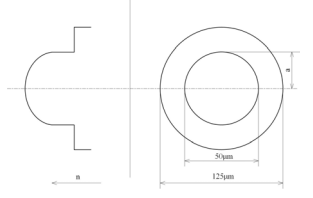
\includegraphics[scale=1]{obrazky/mnohavid2.png}
  \end{center}
\end{figure}

\begin{figure}[!ht]
\begin{center}
    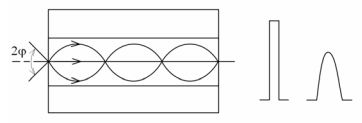
\includegraphics[scale=1]{obrazky/sirmnoh2.png}
  \end{center}
\end{figure}

Charakteristiky tohoto typu vlákna: disperze při 0,85µm cca 1 ns/km, útlum 2,5 - 8 dB/km, šířka přenášeného pásma 600 Mbit


\subsection{Jednovidová vlákna}
Vyznačují velmi malou disperzí, velmi malým útlumem a vysokou přenosovou kapacitou, nacházejí uplatnění především pro dálkové přenosy. V tomto případě se vláknem šíří pouze jeden vid a to ve směru osy. Aby se tohoto stavu mohlo dosáhnout, je zapotřebí zmenšit průměr jádra na hodnotu rovnou jen několika vlnovým délkám světla. \newpage

\begin{figure}[!ht]
\begin{center}
    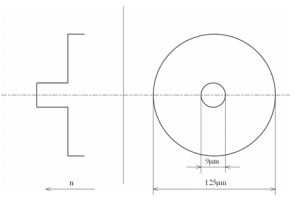
\includegraphics[scale=1]{obrazky/jednovid.png}
  \end{center}
\end{figure}

\begin{figure}[!ht]
\begin{center}
    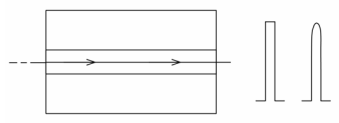
\includegraphics[scale=1]{obrazky/sirjed.png}
  \end{center}
\end{figure}

Charakteristiky vlákna: disperze cca 0,3 ns/km, útlum 0.2 db/km při vlnové délce 1,55µm, šířka pásma 10 Gbit. Průměr jádra = 7 – 9 µm, průměr pláště = 125µm. 

\subsection{Polymerová optická vlákna (POF)}
Současně s rozvojem přenosu po skleněném vláknu byla snaha uskutečňovat i přenosy po vláknech z umělých hmot. Problémem těchto vláken byl a je velký útlum. Původně se pohyboval ve 100kách dB/km, v posledních letech se dostáváme k hodnotám až 10 dB/km. Tato hodnota je již akceptovatelná pro sítě typu vlákno do domu. Současně se podařilo i zvýšit odolnost těchto vláken k teplotě. Současná vlákna odolávají hodnotám 200 až 300°C. 

Velkou předností těchto vláken je jednoduchá a snadná montáž. Snadná a rychlá příprava konektorů přímo v terénu.

\begin{figure}[!ht]
\begin{center}
    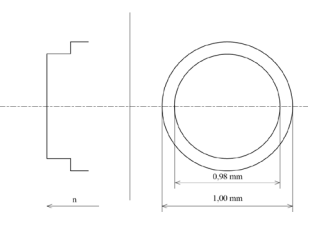
\includegraphics[scale=1]{obrazky/polym.png}
  \end{center}
\end{figure}

Pomocí těchto vláken lze realizovat Gbit Ethernet, případně multigigabitové přenosy do vzdáleností cca 200 m a to v typických přenosových oknech 850 a 1 300 nm.

\clearpage
\section{Výroba optických vláken, druhy vláken a kabelů (standardy ITU-T, G.65x), spojování optických vláken a kabelů, optické konektory.}

\subsection{Výroba optických vláken}
Dvě hlavní metody:
\begin{itemize}
    \item Plynná fáze - tažení ze skleněné preformy
    \item Kapalná fáze - vícesložková vlákna
\end{itemize}

\subsubsection{Plynná fáze}
Představuje moderní technologii výroby. Preforma je v podstatě skleněný polotovar ve tvaru válcové tyčinky, z níž se táhne optické vlákno. Její profil představuje zvětšený profil optického vlákna. Z této preformy se po intenzivním lokálním ohřevu táhne vlastní vlákno. Nato se okamžitě povléká vrstvou z polymeru o tloušťce několika mikrometrů tzv. primární ochrana, aby bylo mechanicky chráněno a ihned se navíjí na buben.

\begin{figure}[!ht]
\begin{center}
    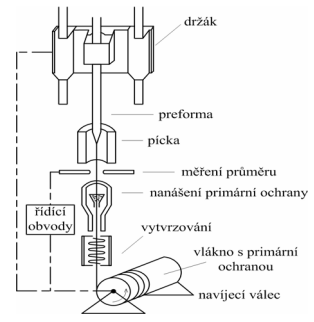
\includegraphics[scale=1]{obrazky/preforma.png}
  \end{center}
\end{figure}

K přípravě preformy metodou depozice (kondenzace) z plynná fáze (CVD) se používají tyto technologie:
\begin{itemize}
    \item OVD (Outside Vapour Deposition), vnější depozice z plynné fáze, při které dochází k boční depozici na jádro rotující konstantní rychlosti.
    \item MCVD (Modified Chemical Vapour Deposition), tzv. modifikovaná chemická depozice z plynné fáze, která patří mezi inside metody, tzn. oxidy jsou nanášeny na vnitřní stěnu rotující ke křemenné trubice
    \item PCVD (Plasma Chemical Vapour Deposition), plazmatická chemická depozice z plynné fáze, při které jsou jako u MCVD deponovány oxidy uvnitř rotující křemenné trubice, avšak reakce dle výchozích rovnic je iniciována mikrovlnnou plasmou
    \item VAD (Vapour Phase Axial Deposition), axiální depozice z plynné fáze, která se liší od předchozích technologií nanášením oxidů na rotující terčík z nosného materiálu v axiálním směru
\end{itemize}

\subsection{Kapalná fáze}
Vícesložková vlákna vychází z klasických sklářských metod. Těmito metodami začínala výroba optických vláken. Základní operace pro výrobu jsou příprava výchozí skloviny, její tavení a tažení vlákna. 

První fázi je tedy příprava ultra čistých výchozích materiálů, většinou práškových oxidů a uhličitanů.

Druhou fází je tavení, kdy získáme homogenní sklo prosté bublinek, přičemž potíže způsobuje především možnost znečištění skloviny z materiálu kelímku a z prostředí pece.

Utavené sklo se po vychladnutí buď obrobí na vhodné rozměry nebo se nechá jen částečně zchladnout a z povrchu se vytáhne tyčinka, čímž se eliminuje znečistění dané obráběním, ale za cenu nižší homogenity skloviny.

Pro vlastní tažení se používají dvě základní metody: metoda "tyčka v trubce" a „metoda dvojitého kelímku“. 

\subsection{Druhy vláken a kabelů}
G.652 je standardní optické jednovidové vlákno 9/125 µm. Tato vlákna jsou nazývána Matched Cladding (MC), vzhledem k typické skokové změně indexu lomu na rozhraní jádra a pláště vlákna. 

G.652.C jako nový typ je dnes k dispozici vlákno typu G.652.C, které lze na rozdíl od běžného vlákna G.652 provozovat v celém rozsahu vlnových délek a využít všechna dostupná přenosová pásma, včetně pásma E (1360 – 1460 nm). To dříve nebylo
možné využít, protože klasická optická vlákna mají v této oblasti zvýšený vložný útlum vlivem rezonancí na absorbovaných iontech vody, které se do vlákna dostaly při výrobě.

G.652.D All Wave vlákno, je kompatibilní se všemi vlákny H.652.

G.653 byla vyvinuta s cílem potlačení chromatické disperze pro vlnovou délku 1 550 nm. Tato vlákna se označují jako vlákna DSF (Dispersion Shifted Fiber). Používají se pro vyšší přenosové rychlosti na velké vzdálenosti s jedinou provozovanou vlnovou délkou. Jakmile však bylo třeba nasazovat v praxi systémy vlnového multiplexu DWDM s více vlnovými délkami, zjistilo se, že tato vlákna mají vedlejší efekt. Ten spočívá v překrývání jednotlivých vlnových délek a vytváření vedlejších parazitních kanálů
a přeslechů.

G.654 byla vyvinuta jako speciální varianta vláken G.652. Tato vlákna jsou optimalizována pro co nejnižší vložný útlum v pásmu 1 550 nm a mají posunutou mezní vlnovou délku (vlnová délka do které fungují jako jednovidová). Jsou nákladná, používají se téměř výhradně k extrémním dálkovým přenosům pro podmořské kabely bez zesilovače na trase.

G.655 s posunutou nenulovou disperzí (NZ-DSF, Non Zero – Dispersion Shifted Fiber) jsou optimalizována pro přenosovou oblast v pásmu 1 550 nm. Tato vlákna se dnes používají především v dálkových optických sítí a na rozdíl od vlákna typu G.653 nemají nulovou disperzi pro vlnovou délku 1 550 nm. Malá nenulová disperze je nutná, aby se zde příliš neprojevovaly vedlejší nelineární efekty. Tento typ vlákna je určen k provozu technologie DWDM a pro vysoké přenosové rychlosti.

G.656 s posunutou nenulovou disperzí (NZ-DSF, Non-Zero Dispersion Shifted Fiber) jsou optimalizována pro přenosovou oblast v pásmu 1 460–1 625 nm. Tato vlákna jsou určena pro systémy vlnového multiplexu DWDM a CWDM. V pásmu S umožňují u systému DWDM až 40 kanálů. Maximální chromatická disperze je stanovena na 2–14 ps/nm/km, maximální polarizační disperze 0,20 ps/km.

G.657.A pro vnitřní kabeláže a pro optické přístupové sítě.

G.657.C nový typ vlákna, které je odolné na mikroohyby, do poloměru 5 mm.

\subsection{Spojování optických vláken a kabelů}
Tak jako metalické kabely, jsou i optické kabely dodávány v určitých délkách (podstatně delších), které je zapotřebí vzájemně napojovat, tedy spojit vzájemně jednotlivá vlákna a poté i plášť. Spojování optických vláken je mnohem složitější než u metalických kabelů, spojky pláště jsou v podstatě shodné se spojkami u plastových kabelů.

V místech, kde bude častěji zapotřebí přerušovat optickou trasu, např. z důvodů měření apod., se zapojují optické konektory. Z tohoto pohledu můžeme tedy spoje ve vláknové optice rozdělit na:
\begin{itemize}
    \item spoje nerozebíratelné
    \item spoje rozebíratelné
\end{itemize}

\subsubsection{Spoje nerozebíratelné}
Do této skupiny řadíme nejčastěji používanou metodu tavného svařování, metody spojování optických vláken lepením a nejnovější metoda pevných metalických spojek. 

Tavné svařování: \\
Ze známých metod se nejvíce ujalo a rozšířilo svařování elektrickým obloukem. Již méně se používá metoda svařování plynovým plamenem nebo laserem CO2. Z důvodu toho, že ve sváru nesmí dojít k zúžení průměru vlákna, jsou tato při svaru posouvány proti sobě. Tyto operace jsou velmi důležité pro vlastní kvalitu sváru a jsou zpravidla kontrolovány automaticky. Mechanická pevnost spojů dosahuje asi 70\% pevnosti vlákna a střední hodnota optického útlumu se pohybuje kolem 0,02 dB

Slepované spoje:\\
U těchto spojů se používá lepidel k přilepení vláken k podkladu a ke spojení vláken dohromady. Lepidlo plní následující funkce:
\begin{itemize}
    \item má velmi podobný index lomu jako vlákno
    \item zajišťuje ochranu spoje před prostředím
    \item trvale zajišťuje vlákna v patřičné poloze
    \item zabraňuje deformacím spoje a zajišťuje pevnost v tahu
\end{itemize}
Nejčastěji používaný typ spojky sestává z trubičky s vnitřním otvorem, jehož světlost odpovídá vnějšímu průměru spojovaných vláken a v níž se dotýkající konce vláken zalepí. Ztráty těchto spojů jsou kolem 0,1 dB, případně i méně. Spoje jsou citlivé na změnu
teploty. Přídavná ztráta 0.1 dB může nastat po teplotním cyklu -30°C - +70°C.

Mechanické spoje: \\
Již z názvu je zřejmé, že osové vyrovnání vlákna se provádí za pomoci různých mechanických struktur, jako jsou V drážky, tunely vytvořené mezi bloky tyček, válečků a rohů čtvercových profilů. Je důležité, aby takto připravená vlákna byla pevně přichycena k vyrovnávacímu povrchu, neboť musí odolávat manipulaci a vlivu prostředí. Pro trvalé dosažení optické ztráty menší než 0,3 dB je zapotřebí použití optického sdružovacího materiálu mezi konci vláken.

\subsubsection{Spoje rozebíratelné}
Spoje rozebíratelné, tzv. konektorované spoje, se většinou používají v ústřednách, případně v místech opakovacích zesilovačů, v menší míře i v kabelových trasách při použití kabelů s páskovou strukturou. 

Princip konektorů spočívá opět v přesném navádění příslušných konců vláknových světlovodů proti sobě, ale problém je komplikován tím, že konečnou optimální polohu je třeba zajistit vhodným mechanickým dorazem a spojením obou části konektoru. Spojovaná vlákna se nesmí dotýkat, aby nedocházelo k oděru čelních ploch.

Ztráty konektorů tohoto typu se pohybují mezi 0,2 až 0,6 dB podle konkrétní konstrukce a použitého materiálu.

\subsection{Optické konektory}
Typy konektorů:
\begin{itemize}
    \item Bionic - jeden z prvních konektorů (1980), podporovaný firmou AT\&T, kuželovitá ferule, vložný útlum 0,5 – 0,6 dB.
    \item SMA - rovněž starší typ konektoru, nezajištěná ferule proti pootočení, aluminiová nebo ARCAP ferule, šroubovací převlečná matice.
    \item FC - standard pro telekomunikace, keramická nebo kompozitní ferule o průměru 2,5 mm, šroubovací převlečná matice s polohováním.
    \item ST - standard pro telekomunikace, aretace proti potočení vodícím kolíkem, odpružená ferule, bajonetový závěr, vložný útlum 0,2 – 0,3 dB.
    \item SC – podporovaný AT\&T, ISO/IEC11801, push-pull provedení, keramická nebo kompozitní ferule, vložný útlum 0,15 dB.
    \item FDDI – párový konektor pro sítě FDDI, push-pull provedení, keramická ferule, vložný útlum 0,2 dB.
    \item ESCON – obdoba FDDI, podporovaný IBM.
    \item E2000 – evropský standard pro telekomunikace, vyvinutý firmou DIAMOND, provedení push-pull, napružený kryt překrývající feruli, vložný útlum 0,2 dB.
    \item MT-RJ – dvojvláknový konektor, slučitelný s RJ 45, podporovaný AMP, HP, Fujikurou, Sicor.
    \item MTP – určený pro páskové kabely (4, 6 až 12 vláken).
    \item VF 45 – dvojvláknový konektor, pro připojení PC, podporuje firma 3M pro system Volotion.
\end{itemize}

\clearpage
\section{Zdroje a detektory záření – jejich parametry a charakteristiky.}
\subsection{Zdroje}
Zdroje záření tvoří jednu ze základních částí optoelektronického telekomunikačního spoje. I když jako zdroj optického záření můžeme v zásadě použít jakýkoliv světelný zdroj, je kupř. použití žárovky pro současné požadavky zcela nepoužitelné a to z důvodů malé energie a nevýhodné vyzařovací charakteristiky. Z toho důvodu byly a jsou v laboratořích zabývající se zdroji záření velmi intenzivně studovány zdroje na bázi pevné fáze generující záření při pokojové teplotě, a to jsou polovodičové zdroje, z nich pak především zájem je soustředěn nejvíce na luminiscenční diody a laserové diody.

Požadavky, které jsou kladeny na optické zdroje jsou především tyto:
\begin{itemize}
    \item co největší účinnost konverze elektrické energie na energii zářivou
    \item generování záření na takových vlnových délkách, kde útlum stávajících optických vláken je nejmenší
    \item generují záření při pokojových teplotách 
    \item mají vysokou spolehlivost a životnost (otázka laserů)
    \item snadnou modulovatelnost v širokém rozsahu, především změnou injekčního (napájecího) proudu
    \item vysokou monochromatičnost resp. koherenci generovaného záření
    \item co nejužší směrovou charakteristiku vystupujícího záření
    \item snadnou zapojitelnost generovaného záření na optické vlákno
    \item v neposlední řadě malé rozměry a váhu
\end{itemize}

Pro optické telekomunikace přicházejí v úvahu tyto druhy zdrojů:
\begin{itemize}
    \item nekoherentní – luminiscenční polovodičové diody (LED – Light Emitting Diode)
    \item koherentní – lasery: především polovodičové (LD – Laser Diode), pro speciální použití i lasery plynové, pevnolátkové a barvivové
\end{itemize}

Pro nenáročnější aplikace tam, kde není zapotřebí dodržet směrovost optického svazku a pro přenosy na kratší vzdálenosti se používají polovodičové zdroje LED. Pro přenosy na větší vzdálenosti tam kde je zapotřebí vyzařovat v úzkém svazku, je zapotřebí přenášet více vlnových délek (vlnový multiplex – WDM), se v zapojení používají laserové polovodičové diody (LD). 

\subsubsection{Luminiscenční diody}
Luminiscenční diody (LED) jsou levné, lehce dostupné, mají dlouhou životnost, snadno se modulují, mají však velkou divergenci výstupního svazku a vyzařují menší výkon (v porovnání s lasery) na všech vlnových délkách vhodných pro telekomunikační přenosy.\newpage

Spektrální charakteristika LED: 

\begin{figure}[!ht]
\begin{center}
    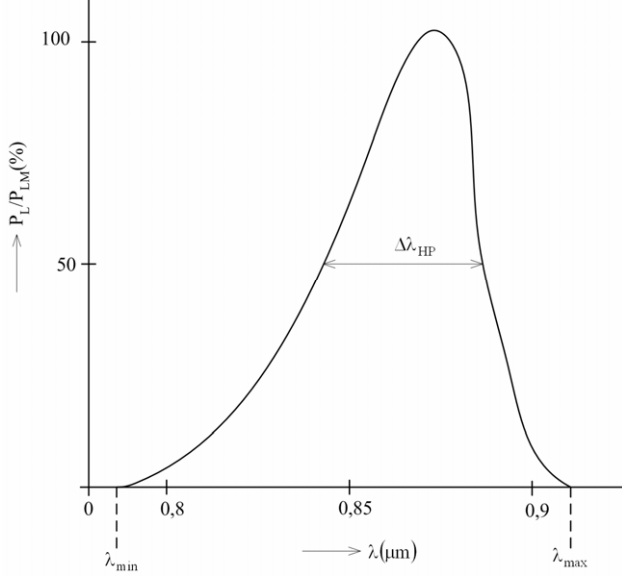
\includegraphics[scale=0.55]{obrazky/spektrLED.png}
  \end{center}
\end{figure}

\subsubsection{Lasery}
Vyznačují se vyšším vyzařovaným výkonem, menší spektrální šířkou, vysokou účinností vazby na vlákno, možností modulovat do vyšších frekvencí (GHz, Gbit/s), na straně druhé však vyžadují vyšší napájení, teplotní stabilizaci, jsou vznikem nejpravděpodobnějších poruch na optických traktech (provádí se zálohování, jejich životnost se však neustále zvyšuje) a jsou dražší. 

Spektrální charakteristika LD:

\begin{figure}[!ht]
\begin{center}
    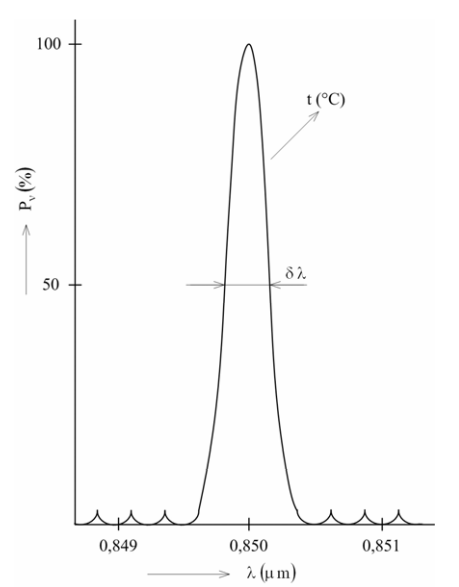
\includegraphics[scale=0.6]{obrazky/spektrLD.png}
  \end{center}
\end{figure}

\subsection{Detektory}
Pro detekci záření se používají prvky zvané detektory. Detektory záření, které jsou potřebné k demodulaci optického signálu v optoelektronických systémech, musí splňovat určité požadavky z hlediska parametrů, slučitelnosti s ostatními prvky, provedení a nákladů. Pro telekomunikační účely se výhradně používají polovodičové detektory. Zájem je soustředěn k polovodičovým diodám, a to především fotodiodám typu PIN a lavinovým fotodiodám APD (Avalanche-Photodiode). Tyto detektory pak musí splňovat následující požadavky:
\begin{itemize}
    \item vysokou citlivost v pásmu výše popsaných světelných zdrojů, tj. pro $\lambda$ = 0,8 až 1,55 µm
    \item musí zaručit dostatečnou šířku přenášeného kmitočtového pásma
    \item rychlou časovou odezvu
    \item malý vlastní šum
    \item minimální rozměry, současně vhodné pro připojení na optické vlákno
    \item necitlivost na teplotní změny, změny napájecího napětí apod.
\end{itemize}

\clearpage
\section{Teoretické problémy přenosu optickou sítí – vlnová a geometrická optika. Nelineární jevy u optických vláken.}

U každého reálného přenosového média a tedy i ve světlovodech dochází ke zkreslení signálu. Toto zkreslení má dvě základní příčiny. Je to jednak nerovnoměrnost kmitočtové charakteristiky vlastního vlákna, která způsobuje změnu spektra signálu a jeho časového průběhu. Druhou příčinou zkreslení signálu a zhoršení jeho rozšiřitelnosti je šum. Úroveň šumu světlovodu se určuje z výkonu na vstupu. Největší roli sehrává šum kvantový, dále se podílí šum tepelný. Vlastní analýza šíření, zvláště v mnohovidových světlovodech je značně složitá. Úkolem analýzy je stanovení impulsní nebo přechodové funkce světlovodu anebo frekvenční charakteristiky.

Problematiku šíření energie v optických vláknech lze řešit dvěma přístupy: buď na základě geometrické, nebo vlnové optiky. 

\subsection{Geometrická optika}
Geometrická optika dává názorné a jednoduché výsledky platné ale jen v prvním přiblížení. Výsledky jsou vhodné především pro mnohovidová vlákna a jejich fyzikální interpretace je snadná, ale neposkytuje úplný obraz o procesech ve vlákně. Geometrická optika vychází z předpokladu, že světelná energie se v prostředí šíří podél určitých křivek – světelných paprsků. Současně předpokládá, že délka vlny šířícího se záření je zanedbatelně krátká ($\lambda$→0). Jako model je uvažováno ideální vlákno, tj. detailně vlákno bez poruch a jejich vliv na uspořádání pole ve vlákně a na šíření energie nemůže proto detailně vystihnout.

\subsection{Vlnová optika}
Vlnová optika dává exaktnější výsledky. Jejich fyzikální interpretace je ale obtížnější a odvozené vztahy jsou mnohdy analyticky neřešitelné. Lze získat přesný obraz o rozložení pole v příčném i podélném směru a odvodit podmínky šíření jednotlivých složek. Vlnová optika příčně homogenních vláken vychází z řešení Maxwellových rovnic. Řešení těchto rovnic umožňuje najít prostorové uspořádání elektromagnetického pole uvnitř i vně jádra a stanovit podmínky šíření pro jednotlivé vidy elektromagnetického pole.

\subsection{Nelineární jevy}
Vznik nelineárních jevů je podmíněn velkými hustotami světelného výkonu ve vlákně. Problém je v tom, že vlákna mají velmi malý průřez jádra a s příchodem systémů vlnového multiplexu se do delších tras začaly začleňovat optické zesilovače, které několinásobně zvyšují výkon ve vlákně. Pokud máme systém pracující s několika desítkami kanálů, tak výkon všech laserů se musí sečíst. Při návrhu tras s přenosovými rychlostmi 10 Gbit.s-1 a víc na jeden kanál je nutno tuto problematiku řešit.

\subsubsection{Stimulovaný rozptyl}
Je nelineární fyzikální jev, při němž dochází k rozptylu světelné vlny srážkami s akusticky nebo tepelně kmitajícími atomy vlákna. Při rozptylu dochází i k mírnému posuvu vlnových délek směrem k vyšším hodnotám. 

\subsubsection{Brilloinův rozptyl}
Je vyvolán podélnou akustickou vlnou vzniklou elektrostrikcí a rozptýlená vlna je spektrálně posunuta o cca 10 GHz. Jeho velikost závisí na úhlu rozptylu, maximum energie je rozptýleno ve zpětném směru. Brillouinův rozptyl je zvláště významný pro signály s úzkou šířkou čáry, a proto je tento jev možné účinně potlačit snížením koherentní délky signálu, neboli rozšířením spektra signálu.

\subsubsection{Ramanův rozptyl}
 Podstatou je vzájemná interakce světla šířícího se v určitém prostředí s tímto prostředím, jejímž důsledkem je frekvenční posuv. Rozptýlená světelná vlna se šíří oběma směry. Kritický výkon závisí opět na materiálu a dále na počtu, středním výkonu a vzájemném odstupu optických kanálů. Na praktické využití Ramanova jevu v telekomunikačních systémech však bylo třeba počkat až do poloviny 80.let, kdy výzkum stimulovaného Ramanova jevu vyústil v jeho praktické nasazení jako zesilujícího prvku, v prostředí jednovidových vláken. 

\subsubsection{Vlastní fázová modulace}
Je výsledkem působení optického impulsu na sebe. Růst a pokles výkonu na hranách optického impulsu vede na změny jeho fáze šíření a tím k jeho tvarovému zkreslení a rozšíření jeho spektra, které může v disperzním prostředí zpětně dále ovlivňovat jeho tvar. Při přílišném rozšíření impulsů pak dochází k jejich překrytí v mezisymbolové interferenci a následně k chybám přenosu.

\subsubsection{Křížová fázová modulace}
Je principiálně podobným jevem jako vlastní fázová modulace, avšak za podmínek, kdy signál jedné vlnové délky fázově moduluje signál vlnové délky jiné. Dochází proto k němu jen u vícekanálových optických systémů.

\subsubsection{Čtyřvlnné směšování}
Je nelineární jev, při němž interakcí signálů dvou a více vlnových délek vznikají signály nových vlnových délek.

\clearpage
\section{Vlnové délky a pásma využívaná pro přenos. Útlum a disperze vláken (disperze chromatická - CD a polarizační – PMD, doporučení ITU). Metody potlačování dispersních vlivů.}

\subsection{Vlnové délky a pásma využívaná pro přenos}
Pro optický přenos informace má význam oblast vlnových délek mezi 0,5–1,6 µm. Především oblast kolem 1,3–1,6 µm vykazuje menší ztráty Rayleighovým rozptylem, minimum hodnot absorpčních ztrát a minimum materiálové disperze. Pro tuto infračervenou oblast existují výkonné zdroje a detektory záření. Do této oblasti rovněž spadá minimální útlum materiálů používaných pro výrobu optických vláken. V oblasti ultrafialového záření pak u většiny těchto materiálů útlum narůstá.

Útlumová charakteristika optického vlákna:
\begin{figure}[!ht]
\begin{center}
    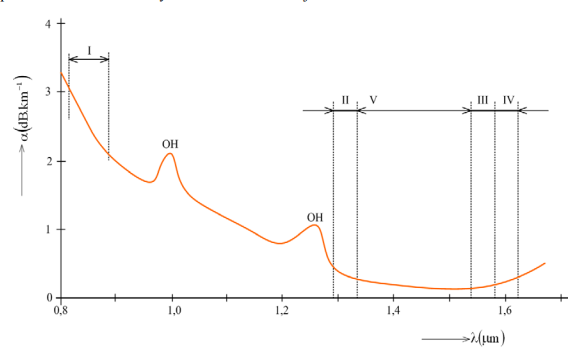
\includegraphics[scale=0.9]{obrazky/okna.png}
  \end{center}
\end{figure}

\subsubsection{I. okno (850 nm)}
Spadá do mnohovidového šíření. Útlumová charakteristika je zde silně klesající a dosahované hodnoty měrného útlumu jsou pro využití zejména v dálkových přenosech příliš vysoké. Díky velmi levným zdrojům záření se přenos využívá u optických přístupových sítí.

\subsubsection{II. okno (1 280 až 1 335 nm)}
Je nejnižší a historicky prvním oknem plně využitelným pro jednovidový přenos na vlákně s průměry 9/125 µm. Typicky dosahovaná hodnota měrného útlumu těsně pod 0,35 dB/km. Toto okno je využíváno pro dálkové přenosy.

\subsubsection{III. okno (1 530 až 1 565 nm)}
Je oknem, ve kterém se u standardního křemenného vlákna nachází minimum měrného útlumu, typicky v hodnotách 0,19 až 0,22 dB/km. Toto okno je využíváno pro dálkové přenosy (transportní a globální sítě).

\subsubsection{IV. okno (1 565 až 1 625 nm)}
Nachází se již za absolutním minimem měrného útlumu, které je však natolik ploché, že se útlumové parametry od III. okna liší jen minimálně. Právě pokrok v technice WDM a optických zesilovačů dovoluje při dálkovém přenosu spojeného spektra III. a IV. okna téměř zdvojnásobit přenosovou kapacitu.

\subsubsection{V. okno (1 335 až 1 530 nm)}
Je pro přenosové využití dostupné teprve od konce 90. let, kdy byly zvládnuty techniky výroby optického vlákna, eliminující příměsi OH natolik, že se ztrácí lokální maximum útlumu na 1 380 nm. Spojená II. až V. okna pak vytvářejí souvislý přenosový kanál o šířce pásma až 50 THz.

\subsection{Pásma}
\begin{figure}[!ht]
\begin{center}
    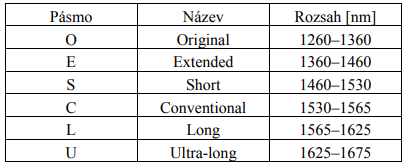
\includegraphics[scale=1]{obrazky/pasma.png}
  \end{center}
\end{figure}

\subsection{Útlum vláken}
Útlum optických vláken je především způsobován:
\begin{itemize}
    \item absorbcí prostředí, v němž se energie šíří
    \item vyzařováním z vlákna
    \item rozptylem na nehomogenitách
\end{itemize}

\subsubsection{Ztráty absorbcí}
Ztráty absorbcí v ultrafialové a viditelné oblasti jsou způsobeny přechody mezi atomárními a v infračervené oblasti mezi molekulárními úrovněmi základního materiálu, příměsí a nečistot, z nichž mají největší vliv ionty kovů Fe, Cu, Cr, jejichž rezonance na určitých kmitočtech je provázena tepelnými ztrátami. Rezonanční kmitočet iontů OH, které tvoří hlavní podíl ztrát, odpovídá vlnové délce 2,8 µm takže leží mimo pásmo využívané pro přenos na optických kmitočtech, avšak druhá harmonická 1,38 µm a třetí harmonická 0,94 µm spadají do oblasti využívaného pásma.

\subsubsection{Ztráty vyzařováním}
Jsou způsobeny lomem šířících se paprsků na rozhraní dvou dielektrických prostředí s různými vlastnostmi, při němž část energie proniká z jádra ven. 

\subsubsection{Ztráty rozptylem}
Jsou způsobeny tím, že molekuly v amorfním materiálu náhodně rozložené tvoří vlastně mikronehomogenity indexu lomu materiálu. Jsou-li tyto nehomogenity a drobné nečistoty rozměrově malé proti vlnové délce, pak rozptylovým ztrátám na nich vznikajícím říkáme Rayleighovy. Tyto ztráty jsou nepřímo úměrné čtvrté mocnině vlnové délky šířícího se záření a rostou velmi rychle směrem k UV oblasti. Charakteristikou Rayleighova rozptylu je jeho všesměrovost.

\subsection{Disperze vláken}
Disperze vln v optických vláknech je hlavní příčinou zkreslení přenášeného signálu. Kmitočtová závislost indexu lomu materiálu, z něhož je světlovod vyroben, je příčinou materiálové disperze.

\subsubsection{Chromatická disperze}
Ve světlovodu se materiálová disperze vidu kombinuje s disperzí vlnovodovou. Výsledný účinek materiálové a vlnovodové disperze bývá
označován jako disperze chromatická. 

Průběh disperze konvenčního vlákna:
\begin{figure}[!ht]
\begin{center}
    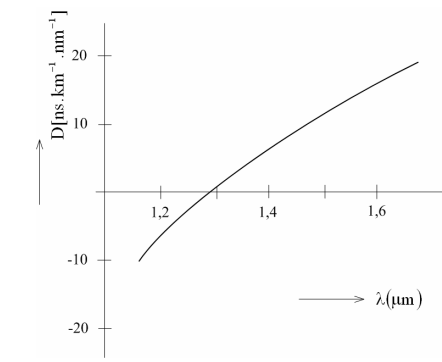
\includegraphics[scale=1]{obrazky/chromdisp1.png}
  \end{center}
\end{figure}

Technologicky se dá připravit vlákno tak, aby i v oblasti vlnové délky 1,55µm se hodnoty disperze snížily k nule. Tato vlákna jsou označována jako vlákna s posunutou disperzní charakteristikou. \newpage

Průběh disperze vlákna s posunutou disperzní charakteristikou:
\begin{figure}[!ht]
\begin{center}
    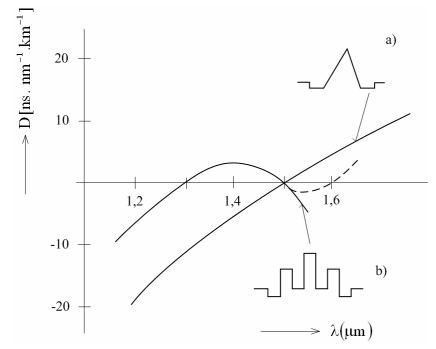
\includegraphics[scale=1]{obrazky/chromdisp2.png}
  \end{center}
\end{figure}

Limitní hodnoty chromatické disperze podle ITU-T G.695:
\begin{figure}[!ht]
\begin{center}
    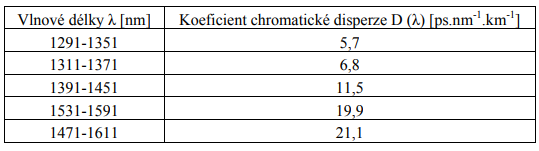
\includegraphics[scale=1]{obrazky/ITUchrom.png}
  \end{center}
\end{figure}

\subsubsection{Polarizační disperze}
S nárůstem přenosových rychlostí v jednovidových optických vláknech nad 2,5 Gb/s vzrostla potřeba měření PMD. Vid, procházející optickým vláknem se nám šíří ve dvou vzájemně na sebe kolmých polarizačních rovinách. Tento jev se nám zhoršuje při jakékoliv kruhové nesymetrii optického vlákna, jenž může být příčina například mikroohyby vytvořenými při vlastní montáži, ale i přímo z výroby nebo při špatném uložení optického kabelu, na který nám poté působí jakýkoli vnější tlak. To vše může mít za následek šíření obou polarizací jinou rychlostí a tím pádem zkreslení signálu nebo rozšíření impulsu. \newpage

Příklad polarizační vidové disperze:
\begin{figure}[!ht]
\begin{center}
    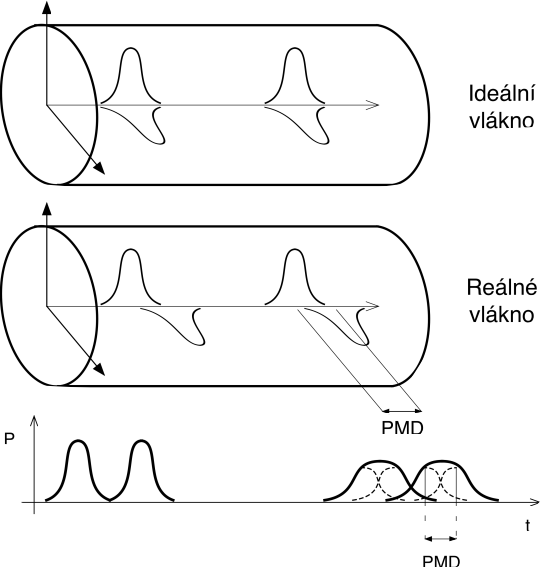
\includegraphics[scale=1]{obrazky/polardisp.png}
  \end{center}
\end{figure}

Limitní hodnoty PMD podle ITU-T G.697:
\begin{figure}[!ht]
\begin{center}
    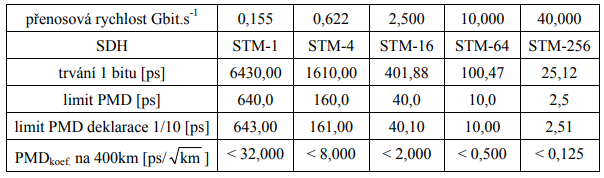
\includegraphics[scale=1]{obrazky/ITUpolar.png}
  \end{center}
\end{figure}

\subsection{Metody potlačování dispersních vlivů}
\subsubsection{Potlačení chromatické disperze}
S nástupem DWDM nastal problém, jak kompenzovat chromatickou disperzi u starších již položených vláken. Nejpoužívanější je pasivní optická kompenzace, ke které se využívají speciální kompenzační vlákna DCF (Disperzion Compensation Fiber) s vysokou hodnotou záporné chromatické disperze. Metoda spočívá v napojení „špulky“ tohoto vlákna na konci trasy (asi 1/6 skutečné délky) a tímto způsobem se vykompenzuje hodnota disperze.

Příklad kompenzace chromatické disperze optotrasy:
\begin{figure}[!ht]
\begin{center}
    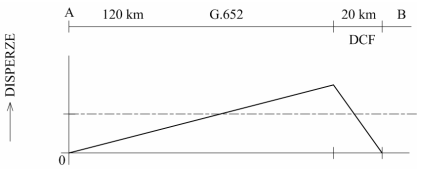
\includegraphics[scale=1]{obrazky/chromkomp.png}
  \end{center}
\end{figure}

V současné době jsou již nabízeny nové typy kompenzačních vláken s dostatečným záporným sklonem disperzní charakteristiky vhodným pro kompenzaci konvenčních i NZDF vláken. Umožňují to např. i speciální mnohovidová vlákna HOM (High Order Mode Fiber). Koeficient chromatické disperze těchto HOM vláken je navíc přibližně 3x vyšší než u klasických DCF vláken, a stačí tudíž oproti nim použít jen třetinu délky kompenzačního vlákna. HOM vlákna mají též nízký měrný útlum a jsou odolná na nelineární jevy. Další možná kompenzace je použití Braggovské mřížky.

\subsubsection{Potlačení PMD}
Omezení hodnot PMD je možné pouze výběrem vláken z kabelu, které mají garantovanou hodnotu. Další možností je pokud se na PMD podílí z největší míry pouze část optické kabelové trasy – provést výměnu kabelové délky.

\clearpage
\section{Optické opakovače a zesilovače.}
Zvýšení dosahu je možné docílit zařazením opakovačů, které mohou být buď se zesílením nebo regenerační. V opakovačích prvního typu se signál zesiluje například v optickém pásmu laserovým zesilovačem. Nedostatkem je zvýšení šumu a tím zhoršení kvality spoje s rostoucí délkou trasy. Opakovače regenerační, ve kterých se signál obnovuje na původní kvalitu, umožňují na základě digitálních přenosů vytvářet spoje, jejichž kvalita není závislá na délce trasy. Použití opakovačů i zesilovačů vyžaduje napájení, což přináší jisté komplikace v případě optických vláken.

\subsection{Opakovače}
V opakovači je světelné záření opět převedeno na elektrický signál, ten je příslušně zesílen, upraven a přiveden na výstup opakovače, zdroj světla (O), který je opět napojen na další úsek optického vlákna.

Přenosový systém s opakovačem:
\begin{figure}[!ht]
\begin{center}
    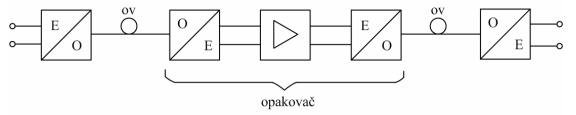
\includegraphics[scale=1]{obrazky/opak.png}
  \end{center}
\end{figure}

\subsection{Zesilovače}
Optické zesilovače (OZ) zesílí příchozí optické záření bez nutnosti konverze na elektrický signál. Jsou to unviersální prvky, zesilující jak analogový, tak i číslicový signál o libovolné přenosové rychlosti. 

Přenosový systém s optickým zesilovačem:
\begin{figure}[!ht]
\begin{center}
    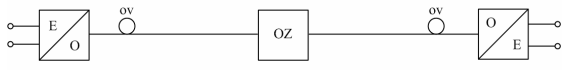
\includegraphics[scale=1]{obrazky/zesil.png}
  \end{center}
\end{figure}

\subsubsection{Optické vláknové zesilovače}
Optické vláknové zesilovače EDFA (Erbium Doped Fibres Amplification). Zesilovač je tvořen tzv. laserovou pumpou a speciálním optickým vláknem, které je dopováno prvky vzácných zemin (Erbiem aj.). Vlivem navázaného zaření z laserové pumpy (o vlnové délce 980 nm nebo 1480 nm) do speciálního vlákna o délce několika metrů, dochází k excitaci atomů dopovaného prvku na vyšší energetické hladiny. Tak je v nich dočasně uložena energie získaná ze záření laserové pumpy. K jejímu uvolnění dochází vlivem přítomnosti přenášeného signálu, jehož energie způsobuje stimulovanou emisi záření o shodné vlnové délce a fázi s přenášeným signálem. Tím dochází k zesílení přenášeného optického signálu. \newpage

Princip optického EDFA zesilovače:
\begin{figure}[!ht]
\begin{center}
    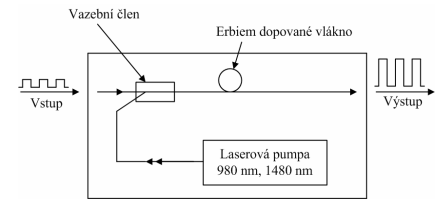
\includegraphics[scale=1]{obrazky/EDFA.png}
  \end{center}
\end{figure}


\subsubsection{Optické Ramanovské zesilovače}
Prakticky se jedná pouze o laserový zdroj záření připojený k optické trase. K zesílení optického signálu se využívá Ramanovského rozptylu na částicích materiálu vlnovodu. Při tomto rozptylu dochází kromě jiného také k přesunu energie z nižších vlnových délek (vlnová délka záření Ramanovské pumpy) na vyšší (vlnové délky přenášeného signálu) a tak k zesílení signálu.

Princip optického Ramanovského zesilovače:
\begin{figure}[!ht]
\begin{center}
    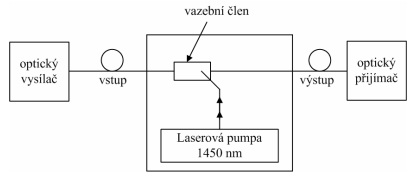
\includegraphics[scale=1]{obrazky/Raman.png}
  \end{center}
\end{figure}


Ramanovský zesilovač se umisťuje na konec přenosového optického vlákna, záření z laserové pumpy se šíří proti zesilovanému signálu. Lze jej využít k zesilování libovolné vlnové délky, stačí jen vhodně zvolit vlnovou délku laserového zdroje (např. 1450 nm pro pásmo 1550 nm). Oba dva druhy zesilovače lze i výhodně vzájemně kombinovat. Tyto zesilovače však zesilují i zkreslení, a tak při dlouhých trasách, je zapotřebí pro obnovu signálu zapojit klasický opakovač. 


\clearpage
\section{Optické přístupové sítě FTTx. Standardy a přenosové rychlosti u pasivních optických sítích (PON).}

\subsection{Optické přístupové sítě FTTx}
FTTx označuje řešení přístupových sítí na základě optických vláken. Je zřejmé, že optický přenos bude získávat na převaze i v přístupových sítích. Z hlediska umístění ukončujících jednotek ONU v optických přístupových sítí a způsobu jejich provedení se rozlišují různé typy optických přístupových sítí:
\begin{itemize}
    \item FTTC (Fibre To The Curb), optická vlákna jsou přivedena k účastnickému rozváděči, k němuž jsou koncové body sítě připojeny metalickými kabely
    \item FTTB (Fibre To The Building), optická vlákna jsou přivedena do budov účastníků, jednotliví účastníci jsou pak připojení pomocí vnitřní sítě
    \item FTTO (Fibre To The Office), optická vlákna jsou zavedena do prostor účastníků s velkými nároky na přenosovou kapacitu
    \item FTTH (Fibre To The Home), optická vlákna jsou zavedena až do účastnických zásuvek
    \item FTTC (Fibre To The Cabinet), optická vlákna zavedena do přístroje (PC)
\end{itemize}

\subsection{Standardy a přenosové rychlosti u pasivních optických sítích (PON)}
V roce 1995 založilo 7 největších světových telekomunikačních operátorů sdružení nazvané Full Service Access Network (FSAN) jejíž cílem byla standardizace a rozvíjení PON sítí. Tyto specifikace byly navrhovány tak, aby uživatelům poskytly plnohodnotné širokopásmové služby jako jsou přenos hlasu, dat a videa.

\subsubsection{APON}
Specifikace G.983.1 APON (ATM Based PON) byla schválena organizací ITU-T v roce 1998. Jedná se o pasivní optickou síť, která pro přenos informací využívá buněk ATM (Asynchronous Transfer Mode). Přenosové rychlosti jsou nabízeny ve dvou variantách: symetrická služba o rychlosti 155,52 Mbit/s a asymetrická služba ve směru ze sítě k uživateli (downstream) 622,08 Mbit/s a ve zpětném směru (upstream) 155,52 Mbit/s. Dodatečně byla doplněna symetrická služba o rychlost 622,08 Mbit/s.

\subsubsection{BPON}
Roku 2001 přijalo ITU-T standard G.983.3 BPON (Broadband PON), který byl vlastně rozšířením předchozího standardu a využívá stejných přenosových rychlostí. Jako přenosového média využívá jednoho či dvou optických vláken G.652. Obousměrná komunikace po jednom vlákně je zajištěna vlnovým dělením. 

\subsubsection{GPON}
V roce 2003 byla v ITU-T schválena specifikace G.984.1 GPON (Gigabit Capable PON), která vychází ze specifikací G.983.X. Především pak rozšiřuje specifikaci G.983.1 ve smyslu rychlosti při zachování principů širokopásmového přístupového systému. Pro přenos využívá ATM buněk, ale také metodu GEM (GPON Encapsulation Method). Tato metoda používá pro přenos GPON rámců, které mají proměnnou délku. ATM buňky i GEM rámce, nebo jejich fragmenty, jsou přenášeny společně v rámcích s pevnou délkou 125 µs. To umožňuje využití paketově orientovaných služeb jako Ethernet či IP (Internet Protocol). Přenosové rychlosti jsou nabízeny ve dvou variantách: symetrická služba o rychlostech 1244,16 Mbit/s, 2488,32 Mbit/s a asymetrická služba ve směru ze sítě k uživateli (downstream) 1244,16 Mbit/s, 2488,32 Mbit/s a ve zpětném směru (upstream) 155,52 Mbit/s, 622,08 Mbit/s, 1244,16 Mbit/s.

\subsubsection{EPON}
Zavedení Ethernetu do přístupových sítí zajistila organizace IEEE přijetím specifikace IEEE 802.3ah. Tato specifikace bývá označována jako EPON (Ethernet Based PON) nebo také EFMF (Ethernet In First Mile Fibre). Cílem bylo zavedení standardu Ethernet až k uživateli a tím zjednodušení navazování lokálních sítí. Pro přenos v obou směrech jsou využívány Ethernet rámce s pevnou délkou 2 ms. EPON je navržen pro mnohabodovou síť sdílející přenosové médium, ale je možno emulovat i komunikaci bod-bod (P2PE Point To Point Emulation). Standardem IEEE 802.3ah jsou specifikovány dva typy rozhraní, které se liší dynamikou a optickými výkony. Typ 1000Base-PX10 je určen pro použití na vzdálenosti do 10 km s maximálním rozbočením 1:16. Typ 1000Base-PX20 je určen pro vzdálenosti do 20 km a rozbočením až 1:32. Přenosová rychlost byla stanovena na 1244,16 Mbit/s symetricky.

\clearpage
\section{Optické linkové zakončení, optické linkové kódy, dosah optického spoje. Optoelektronické linkové trakty. Příklady sítí různých provozovatelů.}

\subsection{Optické linkové zakončení}
Optoelektronické linkové zakončení je určeno k připojení muldexu (multiplexní zařízení) digitálního systému k optickému kabelu. Jeho úkolem je dále převod kódu předepsaného na multiplexním rozhraní (kód HDB3) na linkový kód vhodný pro přenos po optické trase a naopak. Součástí tohoto linkového zakončení jsou též obvody pro dohled a kontrolu signálu.

\subsection{Optické linkové kódy}
Výběr vhodného kódu je důležitým krokem při návrhu systému s optickými vlákny. Nejjednodušší by bylo volit shodné kódy užívané pro metalická vedení. Světlo má však odlišnost v tom, že nemůže nabývat záporných hodnot jako je tomu u standardních kódů. Zápornou polaritu bipolárních kódů AMI nebo HDB3 nelze proto reprezentovat přímo, ale jen zprostředkovaně, buď za pomoci trvalého předpětí třístavovým kódem nebo unipolárním kódem s informačním obsahem větším nebo rovným ternárnímu kódu. Další možností je převod bipolárního signálu na jeho ekvivalentní binární formu s následným přechodem na vhodný linkový kód. Vlastní výběr a návrh kódu souvisí s celkovou koncepcí přenosového systému. V současné době tvoří poměrně rozsáhlou kategorii, takže návrh nového kódového předpisu pro nový systém prakticky nepřipadá v úvahu. Na linkový signál generovaný na základě daného kódového pravidla jsou kladeny tyto požadavky:
\begin{itemize}
    \item vysoký obsah taktovací složky
    \item konstantní ss složka
    \item minimální šířka pásma
    \item možnost jednoduché detekce chybovosti
    \item obvodová jednoduchost kodéru a dekodéru
    \item systémová kompatibilita
\end{itemize}
Vzhledem k charakteru optického přenosu přistupují další požadavky: výkon a linearita modulační charakteristiky zdroje záření, útlum a šířka pásma optického kabelu, citlivost a
šumové poměry detektoru záření.

Pro svoji jednoduchost jsou často využívány kódy NRZ (bez návratu k nule) a RZ (s návratem k nule). Pro vyloučení dlouhé posloupnosti nul a jedniček, je ve vysílači a přijímači zapojeno kódovací a dekódovací zařízení, ve kterém se provádí překódování zprávy. Automatické měření koeficientu chybovosti se provádí pomocí kontrolního součtu parity.

Pro přenos signálu vyšších řádů (PCM) se využívají kódy mBnB, při kterých se každé slovo přenášené zprávy o délce m bitů, definovaným pravidlem překóduje na n bitové slovo (n > m).

Pro přenosové systémy druhého řádu byl vybrán linkový kód typu 1B2B, který vyžaduje dvojnásobnou šířku přenosového pásma, ale jeho obvodové řešení kodéru a dekodéru je poměrně jednoduché.

Při volbě typu kódu 1B2B je možné uvažovat kódy CMI (Codec Mark Inversion), DMI (Differential Mark Inversion), MCMI (modifikovaný CMI) a MDMI (modifikovaný DMI). 

Ukázky linkových kódů:
\begin{figure}[!ht]
\begin{center}
    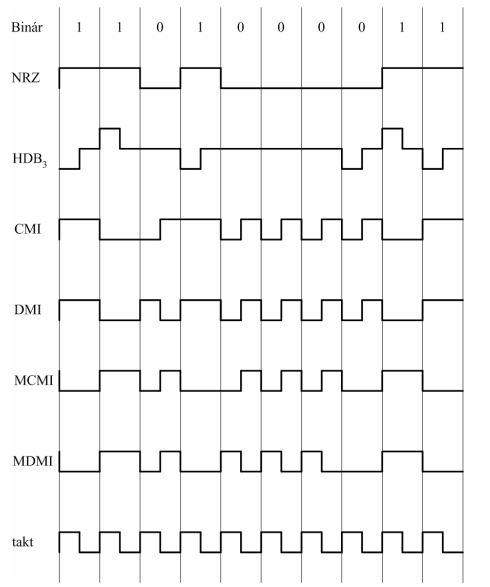
\includegraphics[scale=1]{obrazky/linkody.png}
  \end{center}
\end{figure}

\subsection{Dosah optického spoje}
Dosah optického spoje závisí na útlumu optického vlákna, na zvoleném typu optického zdroje a detektoru, na spojkách, velikosti systémové rezervy, teplotě aj. Dosah optoelektronického linkového traktu je potom dán velikostí opakovacího úseku a počtem regeneračních zesilovačů nebo optických zesilovačů. Při návrhu se vychází z vlastní délky optického spoje, ke které se určí příslušně odpovídající typ vlákna, pochopitleně za respektování příslušné šířky pásma. S volbou typu vlákna by již měla být představa, na jaké vlnové délce bude systém provozován. Dále je zapotřebí provést výběr zdroje a detektoru záření. V neposlední řadě je třeba určit druh modulace, kódování. Pro praktický návrh je důležité znát hodnoty disperze na celém spoji.

\subsection{Optoelektronické linkové trakty}
Optický linkový trakt je vzdálenost mezi vysílačem a přijímačem.

\subsubsection{Optoelektronický linkový trakt digitálního systému druhého řádu}
Optoelektronický linkový trakt druhého řádu je určen pro přenos číslicového signálu s přenosovou rychlostí 8,448 Mbit/s a umožňuje přenos 120 telefonních kanálů. Systém je u nás nasazován do velkoměstských sítí.

Systém se skládá z osmi multiplexních zařízení prvního řádu MX1, dvou muldexů 2. řádu MX2 a optoelektronického linkového traktu OLT2. Ten se skládá ze dvou optoelektronických linkových zakončení 2. řádu OLZ2, přenosového prostředí tvořeného optickými kabely a optoelektronických opakovačů 2. řádu OO2.

V optoelektronickém linkovém traktu jako zdroj záření bývá většinou laserová dioda a jako detektor lavinová fotodioda. Jako linkový kód je použit kód MCMI, takže v zařízení je zapotřebí převodníků kódů HDB3 na MCMI a MCMI na HDB3.

\subsubsection{Optoelektronicky linkový trakt digitálního systému třetího řádu}
Digitální optoelektronický trakt třetího řádu je určen pro obousměrný přenos digitálních signálů s přenosovou rychlostí 34,368 Mbit/s po dvou optických vláknech. Je součástí digitálního přenosového systému třetího řádu, který umožňuje přenos 480 telefonních kanálů, rovněž i přenos dat, rozhlasové modulace a televizního signálu.

Optoelektronický trakt třetího řádu je tvořen dvěma optoelektronickými linkovými zakončeními třetího řádu, optickým prostředím a podle délky spoje opakovači. Celý systém je potom složen na každé straně z 16 multiplexních zařízení 1. řádu. 4 multiplexních zařízení 2. řádu a jednoho multiplexního zařízení 3. řádu.

Pro digitální systémy 3. řádu je předepsán kód HDB2 s přenosovou rychlostí 34,368 Mbit/s.

\subsubsection{Optoelektroniky linkový trakt digitálního systému čtvrtého řádu}
Optoelektronický linkový trakt čtvrtého řádu je určen pro přenosovou rychlost 140 Mbit/s s přenosem po vlákně s gradientním indexem lomu, nebo vláknem jednovidovým, pracujícím nejčastěji na vlnové délce 1,31 µm. Konstrukčně je ve své podstatě obdobou předešlého řešení.

Při použití zdroje LD a vlákna s gradientním indexem lomu, lze dosáhnout vzdálenost mezi opakovači až ke 30 km, při jednovidovém vláknu je mezní hranice k 120 km.

\subsubsection{Optoelektronicky linkový trakt digitálního systému pátého řádu}
Digitální systémy pátého řádu výrazně zvyšují ekonomickou stránku přenosu informací, ale za cenu náročnějších požadavků na technickou stránku zařízení. Tyto systémy jsou vhodné na dlouhé transportní trasy. Jejich přenosová rychlost je 565 Mbit/s a jsou nasazovány na jednovidová vlákna, využívající pracovní oblast vlnových délek 1,31µ a 1,55µm. Ve své podstatě se jedná o sdružení 4 systémů o přenosové rychlosti l40 Mbit/s pomocí časového nebo vlnového multiplexu. Použití jednovidového vlákna klade zvýšené nároky na navazování záření do vlákna, na konektory, na spojky atd. Vysoká přenosová rychlost pak klade velké požadavky na optický vysílač, který musí generovat pulsy s extrémně úzkou spektrální šířkou.

\subsection{Příklady sítí různých provozovatelů}



\clearpage
\section{Multiplexování u optických přenosů – WDM, DWDM, CWDM.}
Současná informační exploze zvyšuje neustále nároky na počty přenášených kanálů a to je důvodem multiplexování signálů na vedení. Existují následující způsoby vícenásobného přenosu:
\begin{itemize}
    \item frekvenční multiplex, jednotlivé signály se přenáší do vyšších kmitočtových pásem, vytváří se tzv. skupiny, které se namodulují na optický signál, generovaný laserem, nebo luminiscenční diodou, Celý multiplexní systém zůstává v oblasti elektronických obvodů a možnosti tohoto vícenásobného přenosu jsou omezené parametry zdrojů světelného záření
    \item časový multiplex, každému signálu je přidělený časový interval, ve kterém je na vysílací straně připojený vysílač a na přijímací straně přijímač daného signálu
    \item elektronický multiplex, po jednom vlákně se nepřenáší binární signál, ale signál vícestavový, čímž stoupne přenosová rychlost n-krát
    \item prostorový multiplex využívá k přenosu více optických vláken pro přenos různých signálů
    \item vlnový multiplex, využívá možnosti vyzařování různých zdrojů světla o různých vlnových délkách, které jsou modulovány jednotlivými informačními zdroji (k přenosu se využívají příslušná "okna" v oblastech minimálního útlumu vláken)
    \item hybridní multiplex, který představuje sloučení vlnového multiplex s elektronickým multiplexem (umožňuje maximální využití přenosových možnosti vlákna)
\end{itemize}
Po stránce využití přenosové kapacity optického vlákna je
nejvýhodnější vlnový multiplex

\subsection{WDM}
Původní vlnový multiplex používá pro přenos pouze dvě, resp. tři vlnové délky většinou v obousměrném provozu na jednom optickém vlákně. Pasivní vlnový multiplexer WDM je jednoduché a levné zařízení. Tyto vlnové multiplexy (couplery) využívají vlnové délky 830, 850, 1300, 1310 a 1550 nm.

Princip vlnového multiplexu:
\begin{figure}[!ht]
\begin{center}
    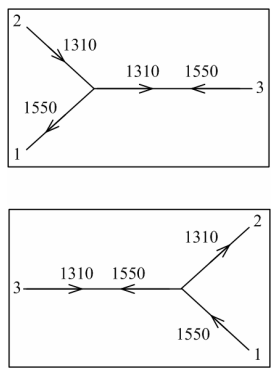
\includegraphics[scale=0.7]{obrazky/multiplex.png}
  \end{center}
\end{figure}
\subsection{DWDM}
DWDM (Dense Wavelength Division Multiplexing) tzv. „hustý“ vlnový multiplex používá minimální odstupy mezi jednotlivými kanály, takže umí do jednoho vlákna implementovat desítky vlnových délek. V těchto případech se využívá jednovidových laserů a úzkopásmových interferenčních filtrů. Při tom je nezbytné zajistit dostatečnou kmitočtovou stabilitu a extrémně úzkou spektrální čáru. Stabilitu laseru zajištujeme buď zvenčí (injekční synchronizací, fázovým závěsem), pomocí rozprostřené zpětné vazby, nebo braggovských zrcadel. Vzhledem k tomu, že selektivita optických filtrů je v nejlepším případě řádově 10 THz, rozčlenění kanálů se musí provádět na mezifrekvenci pomocí elektrických filtrů, tj. v přijímači musí být směšovač a místní oscilátor ve formě kmitočtově stabilizovaného vysoce koherentního zdroje světla.

Pro praktické návrhy je nezbytné počítat s tím, že dosah jednotlivých kanálů bude různý (jsou dost velké rozdíly) a je nezbytné uvažovat s nejhoršími přenosovými vlastnostmi toho jistého kanálu v multiplexu (případně nejhorší kanály nevyužívat). 

\subsection{CWDM}
CWDM (Coarse Wavelength Division Multiplexing) tzv. „hrubý“ vlnový multiplex vznikla jako levnější varianta DWDM. Technologie CWDM je forma vlnového multiplexu, která využívá větší odstup mezi jednotlivými přenosovými kanály, než je tomu u klasické technologie DWDM. V doporučení ITU-T G.671 bylo specifikováno, že CWDM by měl mít odstup jednotlivých kanálů menší než 50 nm a 8 nm pro vlnovou délku 1550 nm.

Všechny vlnové délky CWDM technologie (k dispozici je 18 kanálů) můžeme využít jen s vláknem typu „Metro“ neboli s plným spektrem podle standardu G.652.C. „Metro“ je typ vlákna, které je vyrobeno bez navýšení útlumu v oblasti vlnových délek 1360 až 1450 nm. V běžných případech stávajících optických tras máme ale většinou k dispozici jen standardní optické jednovidové vlákno 9/125um, odpovídající standardu ITU-T G.652, je k dispozici 12 kanálů, s vlnovými délkami 1290, 1310, 1330, 1350, 1470, 1490, 1510, 1530, 1550, 1570, 1590 a 1610 nm. 

\clearpage
\section{Transmisní a reflektometrická (OTDR) metoda měření optických vláken. Metody měření CD a PMD. Dohled (monitoring) optických telekomunikačních sítí.}

\subsection{Reflektometrická (OTDR) metoda měření}
Optický reflektometr OTDR je nejpoužívanějším přístrojem pro montážní a provozní měření mnoha parametrů vláken, kabelů a optických tras. Tímto způsobem lze měřit délku vlákna, jeho homogenitu, útlum svárů, optických konektorových spojek a zároveň umožňuje i lokalizovat poruchy. Optický reflektometr využívá metodu zpětného rozptylu.

Metoda zpětného rozptylu, někdy též označována jako metoda optické reflektometrie v časové oblasti (optical time-domain reflectometry, OTDR), vyhodnocuje závislost zpětně rozptýleného optického výkonu při šíření úzkého optického impulsu měřeným vláknem. Pro měření útlumu využívá Rayleighova rozptylu. Případné Fresnelovy odrazy na bodové poruše nebo na koncích vlákna jsou z hlediska měření útlumu nežádoucím jevem, ale jsou vhodné pro měření délky a pro lokalizaci poruch. Fresnelův odraz nastává při dopadu optického záření na rozhranní dvou prostředí s různým indexem lomu. Taková situace nastane v každém optickém konektoru nebo mechanické spojce a může se objevit i ve svařované spojce.

Výsledek OTDR:
\begin{figure}[!ht]
\begin{center}
    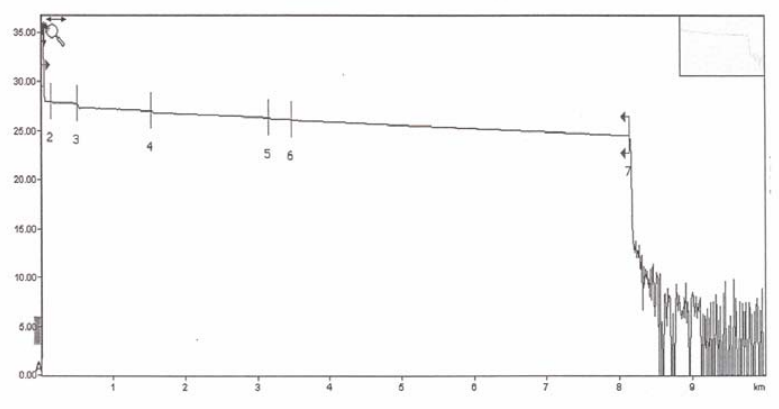
\includegraphics[scale=0.5]{obrazky/zpetroz.png}
  \end{center}
\end{figure}

Odraz je reprezentován výraznou špičkou. Po odrazu vzniká mrtvá zóna. Pro eliminaci mrtvé zóny se používají předřadná vlákna.

\subsection{Transmisní (Přímá) metoda měření}
Kontroluje celkový útlum trasy - spadá sem metoda dvou délek a metoda vložných ztrát.

\subsubsection{Metoda dvou délek}
Měření útlumu metodou dvou délek:

\begin{figure}[!ht]
\begin{center}
    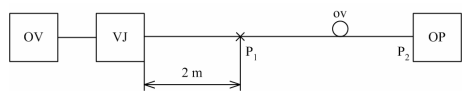
\includegraphics[scale=1]{obrazky/dvedel.png}
  \end{center}
\end{figure}
Tato metoda je pro svoji vysokou citlivost doporučena za metodu referenční (i když se jedná o metodu destrukční). Po navázání optického výkonu ze stabilizovaného optického zdroje (se zapojenou vnitřní nebo vnější vysílací jednotkou V.J. - vazební člen, filtr) do měřeného vlákna o délce 1 se na konci vlákna v bodě 2 změří výkon. Při nezměněných podmínkách vazby se zlomí vlákno přibližně 2 m od počátku (v místě 1) a změří se výkon P1. Dále se vypočte útlum a měrný útlum vlákna. Přesnost metody může dosahovat hodnoty 0,01 dB/km. 

\subsubsection{Metoda vložných ztrát}
Tato metoda také vyžaduje dvoustupňové měření. Jde o metodu provozní a je vhodná zejména pro vlákna a kabely opatřené konektory. Nejprve je třeba provést kalibraci měřící soupravy přímým propojením zdroje s detektorem, čím po změření získáme hodnotu výkonu P1. Měřené vlákno se pak zapojí mezi optický vysílač a měřič výkonu a dostaneme hodnotu výkonu P2. Dále se vypočte útlum a měrný útlum vlákna. V tomto případě se změřený útlum skládá z útlumu vlákna a útlumu spojení měřeného vlákna. Při měření kabelů zakončených konektory je přesnost měření funkcí použitého konektoru a bývá horší než 0,2 dB.

Provozní měření útlumu metodou vložných ztrát:
\begin{figure}[!ht]
\begin{center}
    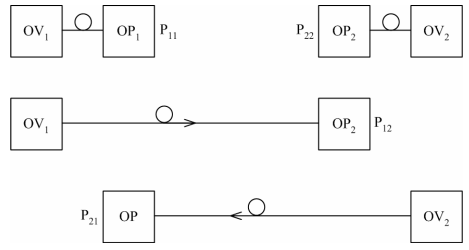
\includegraphics[scale=1]{obrazky/vlozutl.png}
  \end{center}
\end{figure}

V praxi se uplatňuje tato metoda také tak, že na každé straně trasy (A, B) je umístěn jak zdroj (vysílač) tak i měřič výkonu (přijímač). Metoda je čtyřstupňová, dvě měření se nejprve provádí na každé straně připojením měřičů výkonu na zdroje (kalibrace) a dvě měření při připojení měřeného vlákna v obou směrech. Ze čtyř takto získaných hodnot optických výkonů P11, P12, P21, P22 lze vypočítat provozní útlum vlákna.

\subsection{Měření CD}
Používá se metoda fázového posuvu a metoda zpožděných impulsů.

\subsubsection{Metoda fázového posuvu}
Metoda fázového posuvu je dle doporučení ITU-T G.650 udávána jako referenční metoda pro měření chromatické disperze optických vláken. K měření je využit modulovaný zdroj záření o několika vlnových délkách. Na přijímací straně se pro detekci přijímaného testového signálu užívá přístroje pro měření fáze, například vektorvoltmetr. Výstupní změřenou fázi porovnáme se vstupní fází signálu a z jejich rozdílu je stanovena změna fáze signálu po průchodu měřenou optickou kabelovou trasou. Nevýhoda tohoto měření spočívá v nutnosti použít jiného vlákna v kabelu jako referenční trasu, kterou přenášíme informace od vysílače k přijímači o vstupní fázi. 

Metoda fázového posuvu:
\begin{figure}[!ht]
\begin{center}
    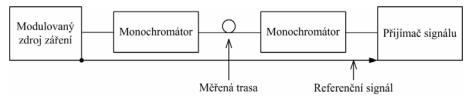
\includegraphics[scale=1]{obrazky/chrommer.png}
  \end{center}
\end{figure}

\subsubsection{Metoda zpožděných impulsů}
Měřící metoda spočívá na vysílání optických impulsů v různých vlnových délkách, ale s přesně stanovenou velikostí impulsu a v přesných rozestupech. Porovnáním rozestupů vstupních impulsů s přijatými na výstupu se určí zpoždění vlivem chromatické dispeze. 

Metoda zpožděných impulsů:
\begin{figure}[!ht]
\begin{center}
    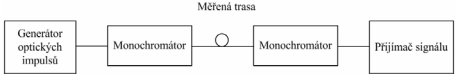
\includegraphics[scale=1]{obrazky/chrommer2.png}
  \end{center}
\end{figure}

\subsection{Měření PMD}
Pro měření PMD se používají 3 metody:
\begin{itemize}
    \item Interferometrická metoda
    \item Metoda skenování vlnové délky
    \item POTDR
\end{itemize}

\subsubsection{Měření PMD interferometrickou metodou}
Tato metoda měření PMD je založena na interferenci (skládání vlnění) nízkokohorentního (koherence - spektrální čistota) optického záření. Na výstupu měřené optické trasy je přímo umístněn interferometr, který nám záření rozdělí do dvou větví. V jedné větvi je pevné zrcadlo a v druhé pohyblivé. Pohyblivým zrcadlem se mění fázový posun mezi přijímanými signály obou větví a za pomoci interference se nám na detektoru ukáže zpoždění vlivem PMD. 

Měření PMD interferometrickou metodou:
\begin{figure}[!ht]
\begin{center}
    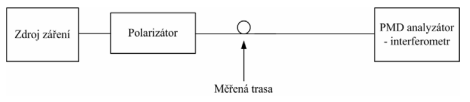
\includegraphics[scale=1]{obrazky/merPMD1.png}
  \end{center}
\end{figure}

\subsubsection{Metoda skenování vlnové délky}
Metoda měření PMD metodou skenování vlnové délky je založeno na principu měření optického výkonu procházejícího danou měřenou optickou trasou v závislosti na vlnové délce. Zdrojem záření může být laditelný laser popřípadě širokospektrální LED dioda. 

Metoda skenování vlnové délky:
\begin{figure}[!ht]
\begin{center}
    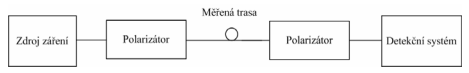
\includegraphics[scale=1]{obrazky/merPMD2.png}
  \end{center}
\end{figure}

\subsubsection{POTDR}
Tato metoda měření PMD kombinuje měření PMD s metodou optické reflektometrie. Tzn. že nám umožní změřit celou trasu a určit případný kritický úsek se zvýšenou hodnotou PMD, který se dá následně vyměnit a tak se dosáhne předepsaných hodnot PMD, (POTDR – Polarization Optical Time Domain Reflectometry).

Metoda POTDR využívá částečně klasické metody měření zpětného rozptylu OTDR. Pracuje na podobném principu, ale metoda POTDR se liší tím, že je reflektogram vyhodnocován polarizovaně. Princip metody – snažíme se vyslat do vlákna trasy měřící signál ve formě sledu impulsů a ze zpětně rozptýleného záření (vliv Rayleighova zpětného rozptylu) se pokusíme vyčíst informace o PMD jednotlivých míst na vláknu trasy.

Metoda POTDR:
\begin{figure}[!ht]
\begin{center}
    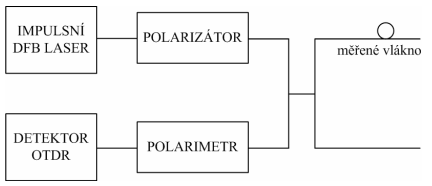
\includegraphics[scale=1]{obrazky/merPMD3.png}
  \end{center}
\end{figure}

\subsection{Dohled optických telekomunikačních sítí}
S rozvojem optických sítí současně vyvstal problém kontroly nad jednotlivými vlákny, celou sítí. Výpadek provozu je možné monitorovat v elektrické vrstvě přenosu. Významní zákazníci (banky aj.), vlastníci „svá pronajatá“ vlákna, mají zájem o dohled přímo nad jejich vláknem a rovněž vyžadují okamžitou informaci o poruše (typ, místo aj.).

Pro tento optický dohled je využívána vlnová délka 1625 nm, která je nad délkami využívanými pro vlastní informační přenosy. Princip může být založen na přímé (transmisní) metodě přenosu nebo s využitím OTDR. Pokles (přerušení přenosu) je detekován a tento poruchový stav je možné přenést na „dispečink“, případně na mobilní telefon odpovědnému pracovníkovi.

Uvedené metody mohou být i kombinovány. Jedním z registrovaných a nejpropracovanějším systémem na trhu je systém MLS (Monitoring Line System).
